\chapter{查询处理框架}\label{chapter:framework}
本章主要介绍两个查询处理框架以分别处理不同应用场景。首先,章节\ref{sec-c3-introduction}阐述了本章的研究思路。其次,章节\ref{sec-c3-interface}介绍了协调者节点和远程结点上的通信接口函数。然后,章节\ref{sec-c3-FTB}介绍了同时利用距离函数上、下界的FTB框架,并给出了实现方案。接着,章节\ref{sec-c3-FLB}介绍了仅利用距离函数下界的FLB框架,并给出了实现方案。最后,小结本章的研究内容。
\section{引言}\label{sec-c3-introduction}
本文的主要研究目标就是降低top-$k$查询时的网络开销,直接将查询轨迹发送到所有远程结点的方式虽然能保证结果的正确性,但网络传输开销消耗较大。为降低这一开销,一个直观的思路是:协调者结点选用合适的降维策略首先对轨迹数据进行降维处理,得到一个概要数据并将该概要数据发送给所有远程结点。远程节点在获取到概要数据后,我们希望根据概要数据能够对查询轨迹和局部轨迹能计算出距离的范围以进行剪枝。此外,我们希望通过降维得到的概要数据具有多粒度特性,即粒度越细,所包含的信息量也越多。同时,所计算出来的距离范围也越精确。通过不断精确的距离范围,我们能进一步剪枝不相关的候选。
整个剪枝过程如图\ref{fig-chapter3-pruningIdea}所示,随着概要数据从粒度1到粒度n的不断传输,整个系统会过滤掉越来越多的候选。这里有两点需要注意:(i)粒度越高,对应的概要数据所能表示的信息量也越接近原始轨迹数据,(iii)在由粗到细剪枝过程中,可能不需要到最细粒度,结果已经找出。
\begin{figure}
	\centering
	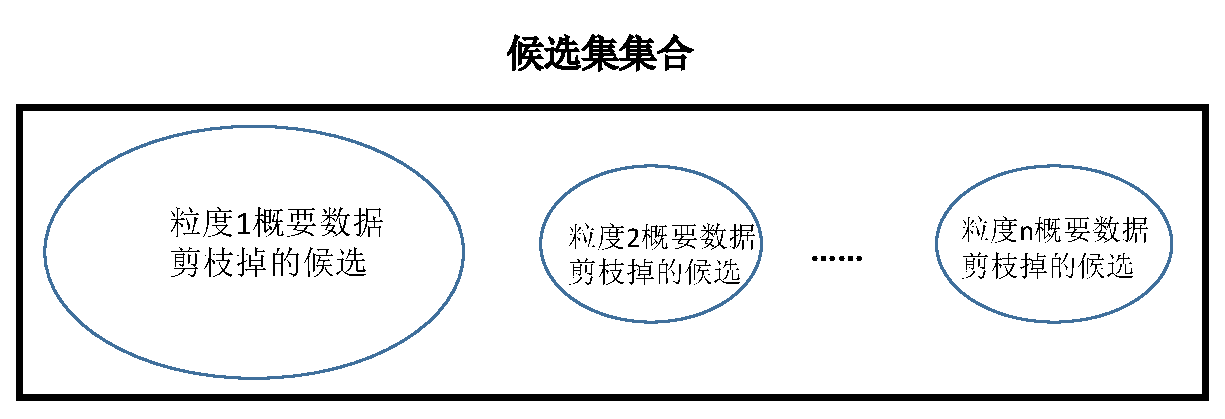
\includegraphics[width=0.73\textwidth]{Fig/chapter3/Idea}
	\caption{逐步剪枝策略}
	\label{fig-chapter3-pruningIdea}
\end{figure}


从以上思路出发,本章从所得到的距离范围出发考虑了两种情况:(i)根据概要数据能同时计算出所给距离函数的上界和下界,(ii)根据概要数据仅能计算出所给距离函数的下界。至于仅能计算出上界的情况不作考虑,这是因为我们需要找的是距离最近的$k$个轨迹。为此,我们首先给出了上、下界特征定义。
\begin{define}界特征(Bound Feature,BF). 界特征,$\langle id, ub,lb \rangle$,记录了一条轨迹的标识($id$),以及它与待查询轨迹的距离上界($ub$)和下界($lb$)。
\end{define}
对任意一条轨迹其默认的距离下界为0,上界为正无穷。我们的目标是不断提高界特征的下界或降低界特征的上界。此外,根据前面所述,我们有时不能同时获得一个较紧的上界和下界。此时,只需使用其保留下界信息。在本章,我们将提出两个查询处理框架。其中前一个框架中将同时使用距离函数的上界和下界。而后一个用来处理仅有下界存在的情况。




\section{接口函数}\label{sec-c3-interface}
在介绍如何进行查询处理框架之前,本节将首先介绍,查询处理所用到的基本通信和处理接口函数。这些接口均为抽象函数,所以在具体应用中,用户可以添加具体的内容(我们再接下来两章将会介绍这些接口函数在使用欧式和动态时间卷曲距离下的具体实现)。我们将这些接口函数按照运行所处位置分为两类。一类是协调者结点上接口函数,另一类是远程结点接口函数。

\textbf{协调者结点函数接口:}
\begin{itemize}
	\item  $\textsf{coordinatorInit}({\cal Q}, {\cal R})$.
	协调者结点运行该函数以实现查询初始化,涉及的内容包含对查询轨迹$\cal Q$进行概要数据计算以及协调者结点跟跟所有远程结点的信息传递。
	
		\item $\textsf{generateInfo}()$. 
		协调者结点生成所需要发送的数据。
	
	
	\item  $\textsf{sendToRemoteSites}(\cal R, x)$.
	协调者节点将数据$x$发给所有在集合$R$中的远程节点。

		\item $\textsf{getFromRemoteSites}(\cal R)$.
		协调者结点从集合$\cal R$中的每个远程结点获取信息。
\end{itemize}	

\textbf{协调者结点函数接口:}
\begin{itemize}
		\item $\textsf{remoteInit}(TS_{r} , S_{r})$.
		远程结点运行该函数以实现初始化,主要工作其为保存在集合$TS_{r}$中的每条轨迹初始化界特征,并将这些特征值放在集合$S_{r}$中。此外,该函数还可能涉及到对每条轨迹数据进行概要数据计算。
		
			\item $\textsf{getFromCoordinator}()$. 
			该函数接受协调者结点运行$\textsf{sendToRemoteSites}$函数时所发数据。
		
			\item $\textsf{sendToCoordinator}(x)$.
			远程结点将信息$x$发送给协调者结点。协调者节点则通过$\textsf{getFromRemoteSites}$函数接受所发消息。
		
			\item $\textsf{updateBounds}(S_r, x)$.
		远程结点根据获取到的信息$x$更新界特征集合中值。
\end{itemize}	
	以上接口函数,为协调者结点与远程结点间的通信提供了保障。接下来的章节,我们将介绍如何利用这些接口函数所传递的信息来进行剪枝。

\section{FTB框架}\label{sec-c3-FTB}
本节将介绍FTB框架的设计原理及实现方案。
\subsection{FTB框架设计原理}
本章第一节提到过,我们假设能对查询对象找到一个数据存储空间较小的概要数据,并利用该概要数据同时计算出距离的上、下界。
FTB框架核心思想就是从这点假设出发,具体的是:使用由粗到细粒度的概要数据,以不断获取更加紧凑的距离上、下界,并以此来进行剪枝过滤。
图\ref{fig-chapter3-FTB}给出了使用多粒度概要数据不断逼近与某一候选轨迹真实距离的过程。图中,横坐标为概要数据的粒度,纵坐标表示相似度距离的值。当概要数据粒度,不断增加的过程中,我们所计算出的相似度上界(红色实线)和下界(蓝色虚线)不断逼近相似度的真实值(黑色实线),并最终等于真实值。当获得了所有轨迹的界特征(上、下界)后,我们就可以使用它们进行剪枝。
\begin{figure}
	\centering
	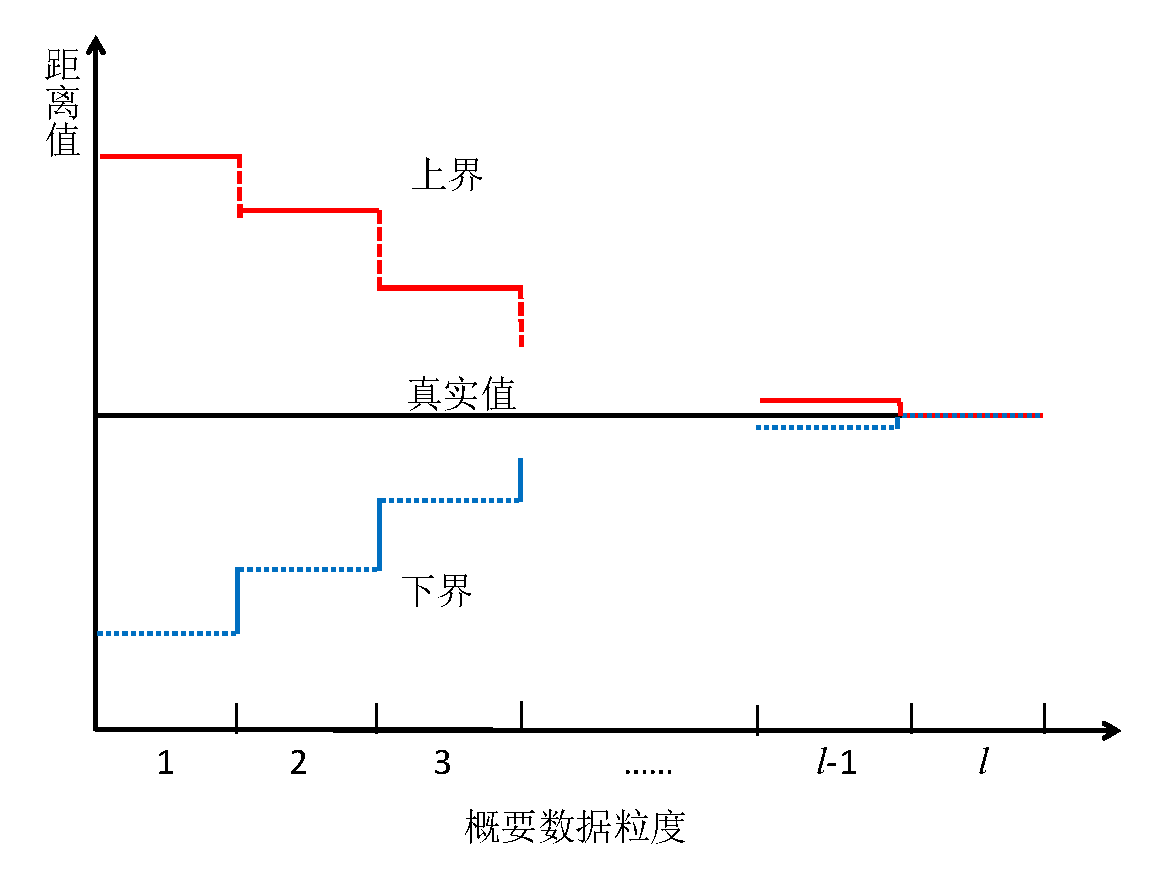
\includegraphics[width=0.73\textwidth]{Fig/chapter3/FTB}
	\caption{多粒度概要数据逼近与某候选轨迹的真实距离}
	\label{fig-chapter3-FTB}
\end{figure}


%\textbf{剪枝原理}:给定一界特征集合$S$,若某一轨迹的下界大于集合中第$k$小的上界,则该轨迹可以被剪枝掉。

\begin{lemma}[\textbf{剪枝原理}]
	给定一界特征集合$S$,若某界特征的下界大于集合中第$k$小的上界,则该界特征所对应轨迹不会进入最终结果集,即可以被剪枝掉。
\end{lemma}
\begin{proof}
	对$S$中的界特征按上界值由小到大排序,并记排序后的第$k$个界特征为$S[k]$。假设某轨迹的特征为$S[c]$($c>k$),且$S[c].lb>S[k].ub$。由于$S[c]$所对应的真实值大于$S[c].lb$,所以有$S[c]$的真实值大于$S[k].ub$。此外,又由于$S[k].ub$大于前$k-1$个界特征的上界,则$S[k].ub$大于前$k-1$个界特征所对应轨迹的真实距离值。因此,$S[c]$所对应的轨迹真实距离值大于前$k-1$个界特征所对应轨迹的真实距离值。故$S[c]$可以被剪枝掉。
\end{proof}
图\ref{fig-chapter3-Bound}展示介绍了剪枝原理。首先,将界特征按上界有小到大拍完序后。对于第$c$个轨迹($c>k$),若其下界大于第$k$个的上界。则该轨迹的真实值必然大于前$k$个轨迹的真实值。由于我们的差值只找距离最小的$k$条轨迹,所以第$c$个轨迹不可能存在于结果集中。此时,根据对其计算出来的上、下界就可以将其从候选集合中移除。

\begin{figure}
	\centering
	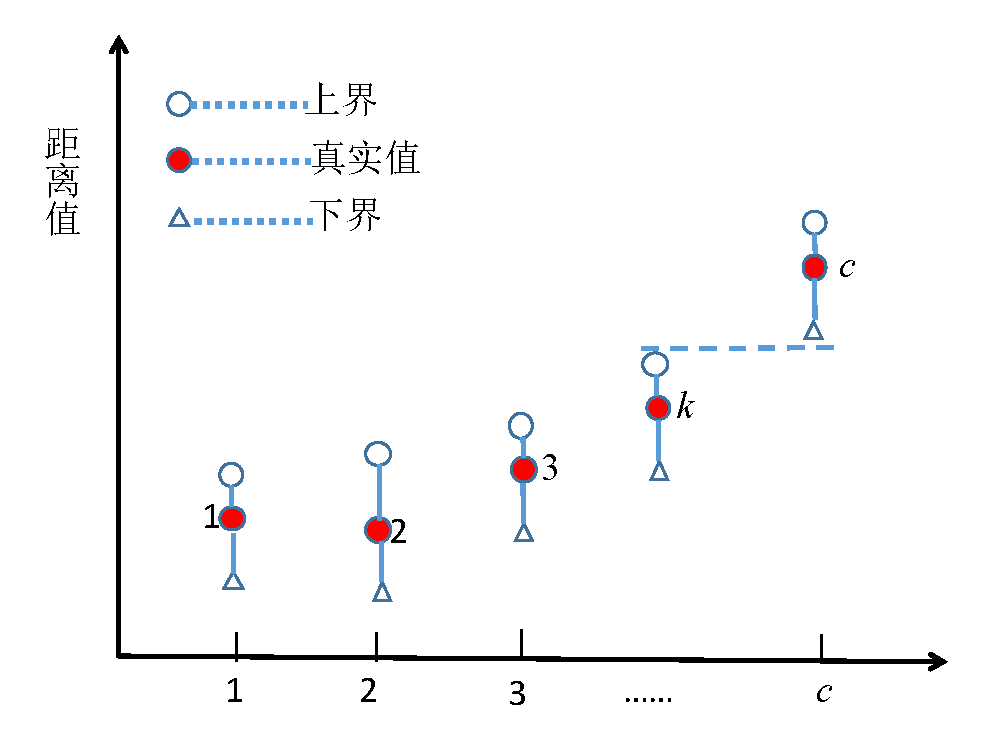
\includegraphics[width=0.73\textwidth]{Fig/chapter3/Bound}
	\caption{剪枝示例}
	\label{fig-chapter3-Bound}
\end{figure}



\subsection{FTB框架实现}
本节将首先介绍FTB(Framework with Two Bounds)框架,以处理那些能同时得到距离上、下界的情况。此外,需要保证当使用最细粒度的概要数据计算上、下界时,上界等于下界。即此时计算出来的上、下界等于距离的真实值。
该框架分为两个部分,一部分是运行在协调者结点的算法1,另一部分是运行在所有远程结点的算法2。在框架运行过程中,这两个部分互相通信并协调工作。整个过程,可以分为3个阶段:初始化阶段,迭代交互式剪枝阶段,最终结果获取阶段。下面将对这三个部分分别进行介绍:

\begin{algorithm}[t]
	\caption{FTB之协调者结点}
	\label{alg:frame1-coordinator}
	\begin{algorithmic}[1]
		\REQUIRE 查询轨迹${\cal Q}$, 结果集大小$k$;
		\ENSURE $k$条最相似轨迹的ID;
		
		\STATE	{${\cal R} \leftarrow$ 远程结点集合;\label{a1:inital}} 
		\STATE	{\textsf{\textsf{coordinatorInit}}(${\cal Q}, {\cal R}$);\label{a1:inital2}} 
		\WHILE{\textbf{true}}
				\STATE {/*生成全局第k小上界*/}
				\STATE {$Info\leftarrow \textsf{generateInfo}()$;}\label{a1:info}\COMMENT {准备概要数据}
				\STATE	{\textsf{sendToRemoteSites}(${\cal R}$, $Info$);\label{a1:sendinfo}}
				\STATE	{$GUBS\leftarrow \textsf{getFromRemoteSites}({\cal R})$;\label{a1:getubs}}
				\STATE	{$gkub\leftarrow argmin_{\tau}(|x\in GUBS, x<\tau|\geq k)$;}
				\STATE	{\textsf{sendToRemoteSites}(${\cal R}$, $gkub$);\label{a1:sendgkub}}
    			\STATE	{/*获取候选集大小${\cal R}$*/}
				\STATE	{$CSS \leftarrow$ \textsf{getFromRemoteSites}(${\cal R}$); \label{a1:getCSS}}
				\STATE	{${\cal R} \leftarrow \{ x.r| x \in CSS, x.|S_{r}| > 0 \}$ }\COMMENT{剪枝远程结点}
     			\STATE	{$sum\leftarrow \sum_{x \in CSS} x.|S_{r}|$;}\COMMENT{候选集大小}
				\IF{$sum ==k$}
					\STATE	{\textsf{sendToRemoteSites}(${\cal R}$, \emph{\textbf{finish}});}
					\STATE	{\textbf{break};\label{a1:finish}} 
				\ENDIF
		\ENDWHILE
		\STATE	{$ids \leftarrow$ \textsf{getFromRemoteSites}(${\cal R}$); \label{a1:finalget}}
		\RETURN $ids$; \label{a1:finalreturn}
	\end{algorithmic}
\end{algorithm}


\begin{algorithm}[t]
	\caption{FTB之远程结点}
	\label{alg:frame1-remote}
	\begin{algorithmic}[1]
		\REQUIRE 局部轨迹集合 $TS_{r}$;;
		\ENSURE 属于top-$k$结果集的轨迹ID;
		
		\STATE	{$S_{r}\leftarrow$局部轨迹界特征集;\label{a2:sr}}
		\STATE	{\textsf{remoteInit}($TS_{r} , S_{r}$);\label{a2:localinitial}}
		\WHILE{\textbf{true}}
				\STATE	{$m\leftarrow \textsf{getFromCoordinator}()$; \COMMENT{从协调者结点获取信息}}
				\IF{$m$ is $Info$} \label{a2:m2Info}
					\STATE	{$S_{r}\leftarrow$ \textsf{UpdateBounds}($S_{r}$, $m$); }
					\STATE	{/* 产生局部最小$k$个上界*/}
					\STATE	{$\widehat{ub}\leftarrow argmin_{\tau}(|x\in S_r, x.ub<\tau|\geq k)$;}
					\STATE	{$S' \leftarrow\{\alpha.ub\,|\,\alpha \in S_{r}, \alpha.ub \le \widehat{ub}\}$} ;
					\STATE	{\textsf{SendToCoordinator}($S'$);\label{a2:mInfoSend} \COMMENT{将最小的$k$个上界返回给协调者结点}}
			\ELSIF{$m$ is $gkub$}	\label{a2:gkub}
					\STATE	{$S_{r}\leftarrow\{\beta\,|\,\beta \in S_{r}, \,\beta.lb \le m\}$ \COMMENT{局部剪枝} }
					\STATE	{\textsf{SendToCoordinator}($\langle r,|S_{r}|\rangle$);}
						\IF{$|S_{r}|=0$}	
							\RETURN;	\label{a2:sendbreak} \COMMENT{当远程结点无候选,则停止运行}
						\ENDIF
			\ELSE %\COMMENT{$m =  \emph{\textbf{finish}}$}
				\STATE	{/* $m$ is $\emph{\textbf{finish}}$*/}
				\STATE	{$ids \leftarrow \{a.id \,|\, a \in S_{r}\}$;\label{a2:finallocal}}
				\STATE	{\textsf{SendToCoordinator}($ids$);}
				\RETURN	; \label{a2:localreturn}
			\ENDIF
		\ENDWHILE
	\end{algorithmic}
\end{algorithm}

\textbf{初始化阶段}: 协调者结点在此阶段执行多种操作,如获取远程结点的列表,概要数据计算以及可能预发送一些信息。在此过程中,我们使用
$\cal R$ 来表示远程结点的集合(算法 \ref{alg:frame1-coordinator}:\ref{a1:inital}-\ref{a1:inital2}  行)。与之对应的,远程结点在该阶段的初始化主要工作是为保存在本地数据集合$TS_{r}$中轨迹初始化界特征并将结果存在局部候选集$S_{r}$ 中。此外,它也会接受协调者结点发过来的数据(算法2:\ref{a2:sr}-\ref{a2:localinitial}行)。
一开始,所有轨迹都是候选。我们把包含候选的远程结点称为候选(远程)结点。


\textbf{迭代交互式阶段}:  在此阶段,协调者结点与候选远程结点交互通信直到剪枝完毕。 首先,远程结点为准好粗粒度的概要数据并发送给所有候选结点(算法 \ref{alg:frame1-coordinator}:\ref{a1:info}-\ref{a1:sendinfo}行)。在接收到概要数据属后,候选远程结点利用该概要数据进行计算距离上、下界并更新界特征。需要注意的是:随着迭代次数的增加,所生成的概要数据粒度越细。这使得我们计算出来的上、下界越来越紧。根据最新的界特征,每个候选结点找出局部最小的$k$个上界并将它们发送给协调者结点 (算法 \ref{alg:frame1-remote}:\ref{a2:m2Info}-\ref{a2:mInfoSend}行)。
当协调者结点获取到所有候选远程结点发送来的上界后,它从中选择第$k$小的上界,记为$gkub$,并将其值发送给那些候选远程结点(算法 \ref{alg:frame1-coordinator} :\ref{a1:getubs}-\ref{a1:sendgkub}行)。候选结点在接受到$gkub$后,就可以剪枝掉局部的一些候选轨迹。具体剪枝做法是,每个局部候选的下界与$gkub$进行比较。如下界大于$gkub$,则将该轨迹从局部候选中删除。剪枝后,候选结点将其所剩候选的个数发给协调者结点。若候选结点的所有轨迹都被剪枝掉,则该结点运行结束(算法 \ref{alg:frame1-remote}:\ref{a2:gkub}-\ref{a2:sendbreak}行)。 在此之后,协调者结点收集候选远程结点所发送的局部候选的个数,并求和计算总的个数。若发现某结点不再包含候选,则将其从候选结点集中移除。此外,若发现当前所剩候选总数正好为$k$个,则迭代终止。协调者将向剩下的候选结点发送终止信号 \emph{\textbf{finish}}。若所剩个数大于$k$,则迭代继续(算法 \ref{alg:frame1-coordinator}:\ref{a1:getCSS}-\ref{a1:finish} 行)。

\textbf{最终结果获取阶段}: 经过上一阶段,最终会剩余$k$个候选。这些候选即为最终的结果。所剩的候选结点在收到上一阶段所发的结束信号后,会将本地所剩候选的ID发送给协调者节点。发送成功后,自身会结束查询(算法\ref{alg:frame1-remote}: \ref{a2:finallocal}-\ref{a2:localreturn}行)。而协调者节点则会收集所有候选结点发送过来的ID,并返回给用户(算法\ref{alg:frame1-coordinator}: \ref{a1:finalget}-\ref{a1:finalreturn}行)。



\section{FLB框架}\label{sec-c3-FLB}
本节将介绍FLB框架的设计原理及实现方案。与FTB框架的不同的是,本框架主要为那些仅能根据概要数据得到距离下界的距离准则而设计。
\subsection{FLB框架设计原理}
针对那些不能同时获得上界的距离度量准则,FTB在使用由粗到细粒度的概要数据以不断获取更加紧凑的距离下界的同时,还不断计算一个越来越紧的全局阈值以剪枝数据。假设与待查询轨迹距离第$k$小的值为$gk$,若某轨迹的界特征的下界大于该值,则该轨迹不会成为最终结果。但$gk$值很难一开始就计算出来。为此,本文的做法是以最小的代价(通信和时间开销)计算$gk$的上界$\theta$,并不断将$\theta$逼近$gk$。然后,在每轮迭代中,用$\theta$来剪枝候选。$\theta$就是我们用来剪枝的全局阈值。
需要区别的是,在$FTB$框架中,是利用界特征的上界进行剪枝。

\begin{figure}
	\centering
	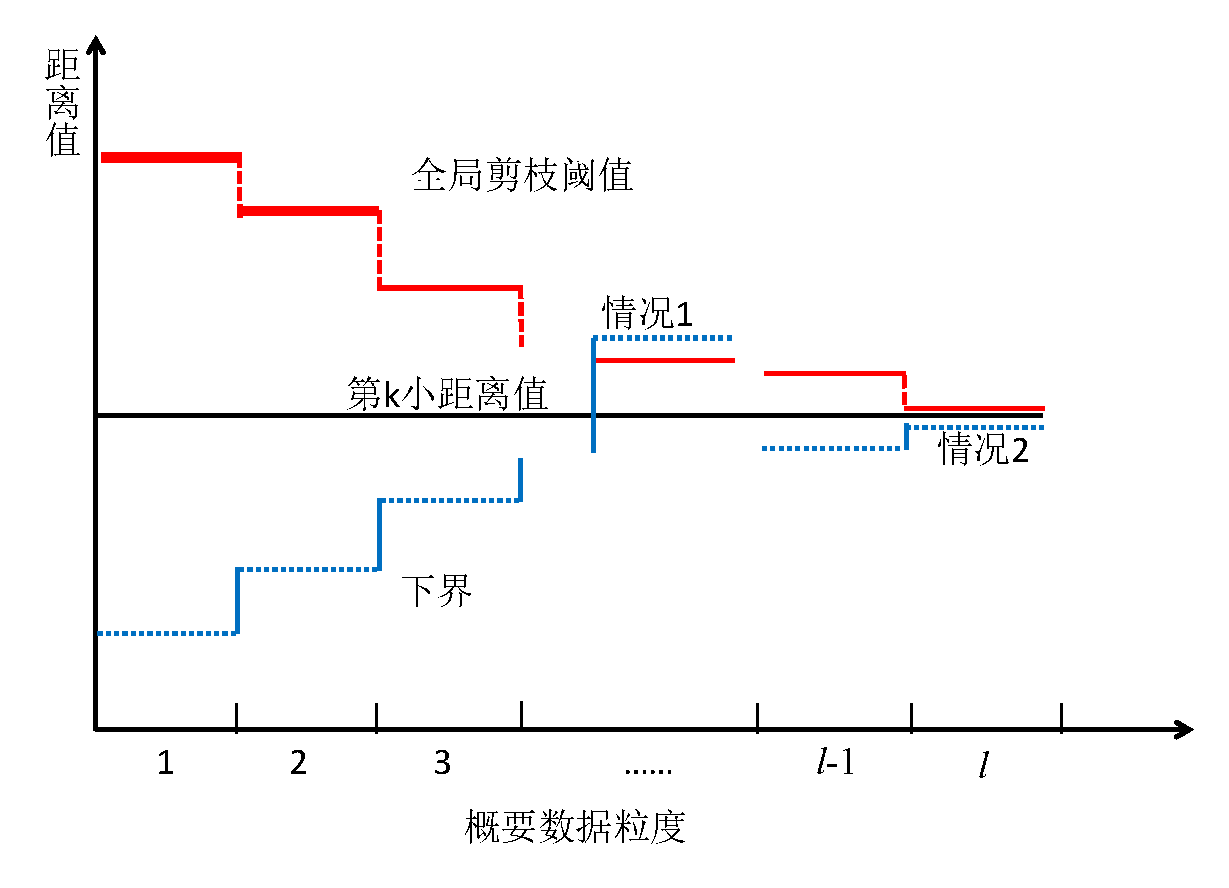
\includegraphics[width=0.73\textwidth]{Fig/chapter3/FLB}
	\caption{利用下界和全局阈值的剪枝过程}
	\label{fig-chapter3-FLB}
\end{figure}

图\ref{fig-chapter3-FLB}示例介绍了,FTB框架对某条轨迹的剪枝过程。图中,中间的黑色直线表示查询轨迹与所有轨迹距离中第$k$小的距离值($gk$值)。
蓝色分段虚线介绍了轨迹距离下界随着概要数据粒度增加,该下界值越来越逼近其真实距离的过程。红色分段实线介绍了全局阈值不断逼近$gk$值。在两者的不断逼近过程中会出现两种情况:第一种情况就是不断逼近过程中,该轨迹的下界大于阈值$\theta$。此时,我们可以将轨迹剪枝掉。第二种情况就是当最细粒度的概要数据后,轨迹的下界仍小于阈值$\theta$。此时,我们将对该轨迹继续保留为候选以待进一步分析。最后,当根据最细粒度的概要数据进行剪枝后,若所保留的候选数仍超过$k$。此时,FTB框架将向包含这些候选的远程结点发送原始轨迹,远程结点则可以计算出真实的距离值并找出最终的$k$个距离最近的轨迹。

\begin{algorithm}
	\caption{FLB之协调者结点}
	\label{alg:frame2-coordinator}
	\begin{algorithmic}[1]
		\REQUIRE 查询轨迹${\cal Q}$, 结果集大小$k$;
		\ENSURE $k$条最相似轨迹的ID;
		\STATE{${\cal R} \leftarrow$ 远程结点集合,${\cal R}' \leftarrow null$;}\label{a3:initialBegin}
		%	\STATE	{${\cal R}' \leftarrow null$;} \COMMENT{${\cal R}'$ 代表已经接受原始轨迹 $\cal Q$的远程结点}
		\STATE	{\textsf{\textsf{coordinatorInit}}(${\cal Q}$,${\cal R}$);}\label{a3:initialEnd}
		\WHILE {\textbf{true}}
		\STATE{$Info\leftarrow \textsf{generateInfo}()$;\label{a3:info}} \COMMENT{生成待发送概要数据}
		\IF{$Info \neq null$}
		%	\STATE	{/*Step 1: 更新全局阈值 $\theta$*/}
		\STATE	{\textsf{sendToRemoteSites}(${\cal R}$, $Info$); \label{a3:sendinfo}} \COMMENT{/*(\ref{a3:sendinfo}-\ref{a3:getTheta}行): 更新全局阈值 $\theta$*/}
		\STATE	{$GLBS \leftarrow \textsf{getFromRemoteSites}({\cal R})$;\label{a3:receiveLowerBounds}} \COMMENT{从远程结点获取局部top-$k$下界}
		\STATE	{$gklbs \leftarrow argmin_{\tau}(|x\in GLBS, x.lb<\tau|\geq  k)$; \label{a3:localtopk}}\COMMENT{选取下界最小的$k$条轨迹}
		\STATE	{${\cal R}'' \leftarrow$ the remote sites  that contain $gklbs$;} \COMMENT{找出包含上述轨迹的远程结点}
		\STATE	{\textsf{sendToRemoteSites}(${\cal R}'' - {\cal R}'$, $\langle {\cal Q}, gklbs \rangle$); \label{a3:sendQ1}} \COMMENT{对未收到$\cal Q$的结点进行处理}
		\STATE	{\textsf{sendToRemoteSites}(${\cal R}'' \cap {\cal R}'$, $\langle null, gklbs \rangle$);\label{a3:sendQ}}\COMMENT{对已收到$\cal Q$的结点进行处理}
		\STATE	{$sv \leftarrow sv \, \cup$ \textsf{getFromRemoteSites(${\cal R}''$)};}
		\STATE	{$\theta \leftarrow argmin_{\tau}(|x\in sv, x<\tau|\geq  k)$;\label{a3:getTheta}}	\COMMENT{选取第$k$小相似度值}	 
		\STATE	{ \textsf{sendToRemoteSites}(${\cal R}$, $\theta$);\label{a3:sendTheta}}
		\STATE	{${\cal R}' = {\cal R}' \cup {\cal R}''$;}
		\STATE {/*Step 2: 剪枝候选远程结点*/}
		\STATE	{$CSS \leftarrow$ \textsf{getFromRemoteSites}(${\cal R}$);\label{a3:BPruneRemote}}\COMMENT{/*(\ref{a3:BPruneRemote}-\ref{a3:EPruneRemote}行): 剪枝并反馈*/}
		\STATE	{${\cal R} \leftarrow \{ x.r| x \in CSS, x.|S_{r}| > 0 \}$;}
		\STATE	{$sum\leftarrow \sum_{x \in CSS} x.|S_{r}|$;}
		\IF{$sum == k$}
		\STATE {\textsf{sendToRemoteSites}($CS$, \emph{\textbf{finish}});} \label{a3:sendFinish} \COMMENT{top-$k$结果已经找到,发结束信号}	 
		%	\STATE	{$ids \leftarrow$\textsf{getFromRemoteSites}(${\cal R}$);}
		\RETURN  \textsf{getFromRemoteSites}(${\cal R}$); \label{a3:EPruneRemote}
		\ENDIF
		\ELSE
		%	\STATE	{从剩余候选结点中寻找top-$k$ }
		\STATE{\textsf{sendToRemoteSites}(${\cal R} - {\cal R}'$, $\langle null, \cal Q \rangle$ );  \label{a3:sendQbegin}} \COMMENT{/*(\ref{a3:sendQbegin}-\ref{a3:return}行):结果提炼*/ }
		\STATE	{\textsf{sendToRemoteSites}(${\cal R} \cap {\cal R}'$, $\langle null, null \rangle$ ); }
		\STATE	{$CSet \leftarrow$ \textsf{getFromRemoteSites}(${\cal R}$); }
		\STATE {$gkSim \leftarrow argmin_{\tau}(|x \in CSet, x.dis<\tau|\geq  k)$;}
		\RETURN  $\{x.id \,| \, x \in CSet, x.dis \le gkSim  \} $; \label{a3:return}
		\ENDIF
		\ENDWHILE
	\end{algorithmic}
\end{algorithm}
\subsection{FLB框架实现}

本节将首先介绍FLB(Framework with Two Bounds)框架,以处理那些仅能获取到下界的情况。
该框架分为两个部分,一部分是运行在协调者结点的算法3,另一部分是运行在所有远程结点的算法4。在框架运行过程中,这两个部分互相通信并协调工作。整个过程,可以分为4个阶段:初始化阶段,全局阈值计算阶段,剪枝阶段和结果提炼阶段。下面将对这四个阶段分别进行介绍:




\textbf{初始化阶段}: 协调者结点在此阶段执行多种操作,如获取远程结点的列表,概要数据计算以及可能预发送一些信息。在此过程中,我们使用
$\cal R$ 来表示远程结点的集合, ${\cal R}'$表示那些已经接受了查询轨迹的结点(算法 \ref{alg:frame2-coordinator}:\ref{a3:initialBegin}-\ref{a3:initialEnd}  行)。与之对应的,远程结点在该阶段的初始化主要工作是为保存在本地数据集合$TS_{r}$中轨迹初始化界特征并将结果存在局部候选集$S_{r}$ 中。此外,它也会接受协调者结点发过来的数据(算法2:\ref{a4:sr}-\ref{a4:localinitial}行)。

\textbf{全局阈值计算阶段}: 该阶段,我们的主要目标是通过迭代通信交互,逐步获取更加精确的全局阈值。在每次迭代中,协调者结点首先发送概要数据给所有候选远程结点
   ( 算法 \ref{alg:frame2-coordinator} \ref{a3:sendinfo}行)。候选远程结点在接受到概要数据后,更新每个候选轨迹界特征值(注:在框架中,界特征只保留ID和下界,无需保持上界)。接着选取局部下界最小的$k$个界特征返回给协调者节点(算法 \ref{alg:frame2-remote}:\ref{a4:receiveInfo}-\ref{a4:sendlowerBounds}行)。其次,协调者选取包含最小的$k$个下界的界特征集合$gklbs$,及包含$gklbs$的远程结点集合${\cal R}''$(算法 \ref{alg:frame2-coordinator}:\ref{a3:receiveLowerBounds}-\ref{a3:localtopk}行)。
   然后,它将待查询轨迹$\cal Q$发送给${\cal R}''$中的远程结点。在发送前,他将${\cal R}''$中的结点分为两类:第一类是接收过$\cal Q$的结点,此时我们需将$\cal Q$ 以及$gklbs$中属于该结点的轨迹发送给对应的结点。第二类是已接收过$\cal Q$的结点,此时,仅需将对应结点的轨迹返回(算法 \ref{alg:frame2-coordinator}:
    \ref{a3:sendQ1}-\ref{a3:sendQ})。当候选远程结点接收到信息这样的成对信息后,针对本地出现在$gklbs$中的轨迹计算出距离值并返回给用户(算法 \ref{alg:frame2-remote}: \ref{a4:localSim}-\ref{a4:sendlocalSim} 行 )。需要注意的是,对于接受成对信息的结点,我们并没有对本地所有候选轨迹计算真实值。其原因是尽管使用全部候选计算出来的距离能有更好的逼近第$k$小距离值,但这样做可能导致时间开销较大,尤其是当数据集中在这些节点上时。远程结点在接收到那些包含$gklbs$的结点发送过来的距离值后,选择最小的值作为全局阈值,并将该值发送给候选结点(算法 \ref{alg:frame2-coordinator}:\ref{a3:getTheta}-\ref{a3:sendTheta}行)。
    
    \begin{algorithm}[t]
    	\caption{FLB之远程结点}
    	\label{alg:frame2-remote}
    	\begin{algorithmic}[1]
    		\REQUIRE 局部轨迹集合 $TS_{r}$;;
    		\ENSURE 属于top-$k$结果集的轨迹ID;
    		
    		\STATE	{$S_{r}\leftarrow$局部轨迹界特征集;\label{a4:sr}}
    		\STATE	{\textsf{remoteInit}($TS_{r} , S_{r}$);\label{a4:localinitial}}
    		\WHILE{\textbf{true}}
    		\STATE	{$m\leftarrow \textsf{getFromCoordinator}()$; }\COMMENT{从协调者结点获取信息}
    		\IF{$m$ is $Info$} \label{a4:update}
    		\STATE	{$S_{r}\leftarrow$ \textsf{UpdateLowerBound}($S_{r}$, $m$); \label{a4:receiveInfo}}
    		\STATE	{$\widehat{lb}\leftarrow argmin_{\tau}(|x\in S_r, x.lb<\tau|\geq k)$;}
    		\STATE	{$S'\leftarrow\{x\,|\,x \in S_{r}, x.lb \le \widehat{lb}\}$; }
    		\STATE	{\textsf{SendToCoordinator}($\langle r, S' \rangle$);\label{a4:sendlowerBounds}}
    		\ELSIF{$m= \langle {\cal Q}/null, gklbs \rangle$}
    		\STATE	{$sv \leftarrow \{ distance({\cal Q},x)|x \in gklbs\}$; \label{a4:localSim}}
    		\STATE	{\textsf{SendToCoordinator}($sv$);\label{a4:sendlocalSim}}
    		\ELSIF{$m=\theta$}\label{a4:pruning}
    		\STATE	{$S_{r}\leftarrow \{ x \,| \, x \in S_{r}, x.lb \le \theta \}$;} \COMMENT{局部剪枝}
    		\STATE	{\textsf{SendToCoordinator}($\langle r, |S_{r}| \rangle$);}
    		\IF{$|S_{r}|=0$} 
    		\RETURN;\label{a4:pruningReturn}\COMMENT{结点不包含候选,则结束}
    		\ENDIF
    		\ELSIF {$m = $ \emph{{\textbf{finish}}}} \label{a4:finishBegin} 
    		\STATE	{$ids \leftarrow \{x.id \,|\, x \in S_{r}\}$;}\COMMENT{收到结束信号,则返回候选ID并结束}
    		\STATE	{\textsf{SendToCoordinator}($ids$);}
    		\STATE	{\textbf{return};\label{a4:finishEnd}}
    		\ELSE \label{a4:ForceExitBegin}
    		%	\STATE	{/*$m= \langle null, \cal Q \rangle$ or $m= \langle null, null \rangle$*/}
    		%	\STATE	{$result \leftarrow \{\langle x.id, distance(x, Q)\rangle  \,  |\, x.id \in S_{r}  \}$;}
    		\STATE	{\textsf{SendToCoordinator}($\{\langle x.id, distance(x, Q)\rangle  \,  |\, x.id \in S_{r}  \}$);}
    		\RETURN;\label{a4:ForceExitEnd}
    		\ENDIF
    		\ENDWHILE
    	\end{algorithmic}
    \end{algorithm}
    
\textbf{剪枝阶段}: 该阶段主要利用$\theta$和下界进行剪枝。当候选远程结点接收到$\theta$后,将会将下界小于所接收的阈值的轨迹从候选集中删除。剪枝完毕后,该结点会将所剩候选数发送给协调者结点。此外,当该结点不再包含任何候选时,则停止运行(算法 \ref{alg:frame2-remote}:\ref{a4:pruning}-\ref{a4:pruningReturn}行)。协调者结点在接收到
所有候选远程结点发送过来的候选数后,计算出总的所剩候选数。若所剩候选总数正好为$k$个,则说明所有候选已经找出。协调结点向候选远程结点发结束信号并等待接收最终结果的ID(算法 \ref{alg:frame2-coordinator}:\ref{a3:sendFinish}-\ref{a3:EPruneRemote}行)。候选远程在接收到结束信号后,则将本地候选的ID发送给协调者结点(算法 \ref{alg:frame2-remote}: \ref{a4:finishBegin}-\ref{a4:finishEnd}行)。若所剩候选总数仍超过$k$,则迭代执行第二和本阶段任务直到$k$个候选被找出或概要数据发送完毕。


\textbf{结果提炼阶段}: 由于界下界最终不一定能逼近到原始距离值,且全局阈值不一定能逼近到第$k$小距离值。所以存在着当概要数据发送完毕,所剩候选数仍超过$k$的情况。此时,需要对剩下的候选进行甄别。FLB框架的做法是将查询轨迹$\cal Q$发送到剩下的候选结点中,并对所有剩余候选计算真实的距离值以找出最终的$k$个结果(算法 \ref{alg:frame2-remote} :\ref{a3:sendQbegin}-\ref{a3:return}行)。需要注意的是在发送$\cal Q$时,若某候选已经接收过$Q$则无需再次发送。

\section{本章小结}\label{sec-c3-FrameCMP}
本章首先介绍了使用概要数据计算距离界特征,并利用特征剪枝的思想。然后介绍了FTB框架以处理那些能根据概要数据同时计算出上、下界的距离函数。进一步的介绍了FLB框架以处理仅能根据概要数据计算出下界的距离函数。对比FTB和FLB两个框架的介绍,我们可以发现两者的共同点都是计算一个全局值来和轨迹下界来剪枝。它们的区别是FTB框架计算出的全局值是从候选轨迹的上界中选取出来的,而FLB框架是对某些轨迹计算真实的距离值,并从这些距离值中选取出来的。所以,尽管FLB框架也可以应用于能同时获取上、下界的距离函数,由于其计算全局阈值需要额外的计算和通信开销。故对于能同时根据概要数据计算上、下界的距离函数,我们使用FTB框架来处理。


\clearpage
\phantom{s}
\clearpage